\documentclass{article}
% Competition/workshop paper, non-anonymous (single-blind) camera-ready: the official style
% requires a track option together with [final]; [final] alone leaves the track name undefined.
\usepackage[sglblindworkshop,final]{neurips_2026}
\workshoptitle{Smart Buildings Challenge (SB26)}
\usepackage[utf8]{inputenc}
\usepackage[T1]{fontenc}
\usepackage{url}
\usepackage{booktabs}
\usepackage{amsfonts}
\usepackage{amsmath}
\usepackage{nicefrac}
\usepackage{microtype}
\usepackage{xcolor}
\usepackage{graphicx}
\usepackage{algorithm}
\usepackage{algpseudocode}
\usepackage{multirow}
\usepackage{array}
\usepackage{tikz}
\usetikzlibrary{positioning,arrows.meta,calc}
\usepackage{enumitem}
\usepackage[font=small,skip=4pt]{caption}
% Compact lists: the main text uses bullets for scanning, within six pages.
\setlist{nosep,leftmargin=1.2em,beginpenalty=10000}
\setlist[itemize,2]{leftmargin=1.1em,label=\textendash}
\usepackage{hyperref}  % after float/algorithm so caption anchors are not duplicated
\input{results_macros}
% Figure include that degrades to a visible placeholder when the file is not built yet.
\newcommand{\figfile}[2]{\IfFileExists{#2}{\includegraphics[width=#1]{#2}}{\fbox{\parbox{#1}{\centering\textbf{??} missing figure \texttt{\detokenize{#2}}}}}}

\title{Schedule-Aware Demand-Based Reset: A Structured Rule-Based Controller for Cross-Building HVAC Transfer in the Smart Buildings Challenge}

\author{%
  Neel Sirivara\\
  University of Washington\\
  \texttt{nsiriv@cs.washington.edu}
}

\begin{document}

\maketitle

\begin{abstract}
The NeurIPS 2026 Smart Buildings Challenge asks for one HVAC control policy that operates procedurally generated commercial buildings it has never seen, under 30-day weather strips from five climates, trading occupant comfort against energy cost and carbon. We present SADR (Schedule-Aware Demand-based Reset), a pure-numpy rule-based controller that reads the plant topology from the building metadata and is otherwise built from physics shared by every generated building. SADR gates its mode on occupancy and schedule with a self-tuning optimum start, regulates each zone with a PI loop on \emph{net heat}, translates heat into damper and valve commands through the supply-air and discharge physics, and resets pressures and hot-water temperature from zone demand. On the 30 public scenarios the final version (v10) scores \REigConfPubCand{} on the leaderboard metric (lower is better), against \MetricPidWater{} for the strongest organizer baseline. Eight development rounds each shipped only under a rule fixed in advance and confirmed on scenarios no decision touched; the last lowers the loss by \REigConfHarshCTwoRelAbs{} on \REigConfHarshCTwoN{} unseen harsh-weather scenarios (\REigConfHarshCTwoWins{} wins). Submissions of fixed versions to Kaggle show that the hidden buildings behave like the public ones and that the hidden weather is harsher. We release the controller and report where it still loses: deep cold, where gas dominates.
\end{abstract}

\section{Introduction}

Learned building controllers have been studied for two decades, yet few run in real buildings; the recurring obstacles are data-hungry training, fragile robustness and poor generalization across buildings~\citep{wang2020rl}. The Smart Buildings Challenge (SB26) isolates the last of these. A submission is a single policy class, instantiated on held-out buildings drawn from the same procedural generator as six public ones and scored on 30-day episodes under weather strips it has not seen~\citep{sb26kit}. The observation and action vectors change shape with the building ($K$ air handlers and $V$ zones expose $K{+}1$ on/off commands and $3K{+}2{+}2V$ continuous setpoints), and the simulator is Google's open-source Smart Buildings simulator~\citep{goldfeder2023lightweight,goldfeder2025suite}.

We take the position that the right first entry in such a benchmark is a \emph{structure-aware rule-based controller}: one that reads the plant topology from the metadata and otherwise encodes physics every generated building shares. It transfers by construction and shows which part of the score is reachable without learning.

\paragraph{Contributions.}
\begin{itemize}
\item \textbf{Design facts} from an analysis of the SB26 reward and plant (Section~\ref{sec:env}).
\item \textbf{SADR}, a deterministic numpy controller built from them (\PolicyMsOurs{}\,ms per step; Section~\ref{sec:method}, Figure~\ref{fig:sadr}).
\item \textbf{A shipping protocol}: screens, loss decompositions and pre-registered full-length confirmations on scenarios no decision touched, with Kaggle submissions used to find which local set predicts the hidden scenarios (Section~\ref{sec:results}, Table~\ref{tab:rounds}).
\item \textbf{An account of where the loss sits} and where SADR still loses (Section~\ref{sec:analysis}); every number is generated from the result files.
\end{itemize}

\section{Environment and metric}
\label{sec:env}

\begin{itemize}
\item \textbf{Plant.} Air handlers (AHUs) serve up to ten zones each through one VAV box per zone, mix return with outside air (recirculation $r\le 0.7$) and can only cool: the supply is $\min(\text{mixed}, \text{SAT})$. Zone flow is $d\,F_{\max}\sqrt{P/P_{\text{design}}}$ for damper $d\in[0.1,1]$ and static pressure $P\in[200,2000]$\,Pa. Fan power is $\text{flow}\times P/\eta$, so it grows as $P^{3/2}$ once dampers are open, and the chiller's COP is a constant 3.5. Heat comes only from the VAV reheat coils on one gas boiler loop (supply 310--350\,K, 0--20\,bar), whose effectiveness $\min(1, C_w/C_a, (308.15-T_{\text{sa}})/(T_w - T_{\text{sa}}))$ caps the discharge at 308.15\,K. Gas is billed as heat delivered plus a tank loss.
\item \textbf{Reward.} Each 5-minute step pays $0.6\,\text{(comfort shortfall)} + 0.2\,\text{(normalized energy cost)} + 0.2\,\text{(normalized carbon)}$. The comfort shortfall is the occupancy-weighted productivity loss: a deviation of $\Delta$\,K from the band costs $\Delta/5$ up to 5\,K and $1+((\Delta-5)/5)^2$ beyond, normalized by total occupancy. It is therefore \emph{zero whenever nobody is in the building}. Occupants are present only on weekday comfort hours (arrivals 06--12, departures 13--19, none on US holidays), and only the building-wide count is observed. The band is 294--297\,K in comfort hours and 289--298\,K otherwise.
\item \textbf{Energy prices.} Energy is normalized by a plant maximum that scales with $K$. In metric units one kW of electricity costs about $2.1\times$ one kW of gas, and one kW of chiller cooling about $0.6\times$.
\item \textbf{Metric.} The leaderboard metric is the mean over scenarios of $|\text{mean per-step reward}|$; lower is better. It is dominated by the extreme climates: the organizers' \texttt{pid\_water} loses \ExtremeRatioFairbanks$\times$ its mild-climate mean in Fairbanks.
\item \textbf{Baselines.} The kit ships \texttt{bang\_bang}, \texttt{fixed\_setpoint}, \texttt{pid} (per-AHU PID on the mean served-zone temperature, plant idle outside work hours) and \texttt{pid\_water} (\texttt{pid} plus worst-zone tracking, a proportional economizer, proportional reheat and a hot-water reset). \texttt{pid\_water} is the strongest and our main comparison; there is no learned baseline.
\end{itemize}

\section{Method: SADR}
\label{sec:method}

SADR is a single \texttt{TransferPolicy} class. Its only state is per-zone integrals, per-AHU dwell counters and the optimum-start statistics, and all gains live in one parameter dictionary (Table~\ref{tab:params}, Appendix~\ref{app:tuning}). Figure~\ref{fig:sadr} shows one control step; Algorithm~\ref{alg:sadr} (Appendix~\ref{app:figs}) gives it in full.

\begin{figure}[t]
\centering
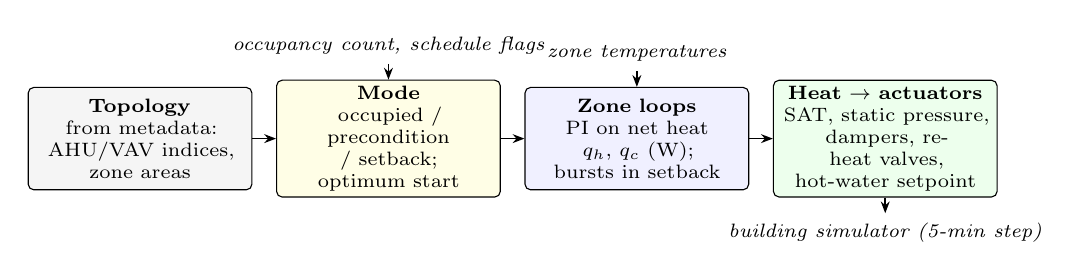
\begin{tikzpicture}[font=\scriptsize, node distance=3mm,
  box/.style={draw, rounded corners=2pt, align=center, inner sep=2pt, minimum height=13mm, text width=27mm},
  arr/.style={-{Stealth[length=1.5mm]}, semithick}]
\node[box, fill=gray!8] (topo) {\textbf{Topology}\\ from metadata:\\ AHU/VAV indices,\\ zone areas};
\node[box, fill=yellow!10, right=of topo] (mode) {\textbf{Mode}\\ occupied / precondition\\ / setback;\\ optimum start};
\node[box, fill=blue!6, right=of mode] (zone) {\textbf{Zone loops}\\ PI on net heat\\ $q_h$, $q_c$ (W);\\ bursts in setback};
\node[box, fill=green!7, right=of zone] (act) {\textbf{Heat $\to$ actuators}\\ SAT, static pressure,\\ dampers, reheat valves,\\ hot-water setpoint};
\draw[arr] (topo) -- (mode);
\draw[arr] (mode) -- (zone);
\draw[arr] (zone) -- (act);
\node[above=2mm of mode, font=\scriptsize\itshape] (occ) {occupancy count, schedule flags};
\draw[arr] (occ) -- (mode);
\node[above=2mm of zone, font=\scriptsize\itshape] (tz) {zone temperatures};
\draw[arr] (tz) -- (zone);
\node[below=2mm of act, font=\scriptsize\itshape] (b) {building simulator (5-min step)};
\draw[arr] (act) -- (b);
\end{tikzpicture}
\caption{One SADR control step. The topology is read once from the metadata; the mode, zone loops and actuator translation run every step. Every gain scales with the zone's floor area (v6), so nothing depends on the size of the building.}
\label{fig:sadr}
\end{figure}

\begin{itemize}
\item \textbf{Topology from metadata.} Index tables come from the observation field names, the positional AHU action lists, the per-VAV action indices and the AHU-to-zone assignments; ranges and statistics come from the normalization metadata. Every action slot is written and clipped on every step. Nothing depends on the number of zones or handlers, the floor plan or the strip; non-finite inputs fall back to schedule values; there are no files, no network and no randomness.
\item \textbf{Modes.} \textsc{Occupied} when the \texttt{comfort\_mode\_now} flag is set and the building is not detected as closed; \textsc{Precondition} when unoccupied but comfort hours start within a lead time (or \texttt{comfort\_mode\_soon}); \textsc{Setback} otherwise.
  \begin{itemize}
  \item ``Somebody is here'' is detected relative to the running minimum of the affinely normalized occupancy count. A weekday on which nobody has arrived by \ParHolidayCheckH{}:00 is a holiday in the kit's occupancy model and is treated as unoccupied until the count rises.
  \item The optimum-start lead is $\ell = \ell_0 + \text{deficit}/(\hat{r}/s)$: the worst zone's distance from the comfort band over a recovery-rate estimate $\hat{r}$ (K/h), re-estimated from each morning's recovery (exponential average, weight \ParRateEma), with safety factor $s=\ParLeadSafety$, clipped to $[\ParLeadMinH, \ParLeadMaxH]$\,h.
  \end{itemize}
\item \textbf{Zone loops on net heat.} Each zone has heating and cooling targets: the sensor band shrunk by \ParMarginOcc\,K (occupied) or \ParMarginPre\,K (preconditioning). Two PI loops compute requested net heat $q_h = k_q (T_h^\star - T)^+ + I_h$ and cooling $q_c = k_q (T - T_c^\star)^+ + I_c$ in watts ($k_q = \ParKqWPerK$\,W/K, integral gain \ParKiWPerKStep\,W/K per step). The integrals unwind past the target, so a zone inside the band free-floats, and the larger request wins.
  \begin{itemize}
  \item \emph{Why net heat, not flow.} The zone-air node responds within minutes. A flow-proportional controller with a 5-minute step oscillates, whereas a net-heat gain of the order of the air node's conductance to the slab is stable, and the integral carries the steady load.
  \item \emph{Setback bursts.} A running handler pays the ventilation load of every zone it serves. The floor (eco band widened by \ParNightLowExt{}/\ParNightHighExt\,K) is therefore held by requesting \ParQSbW\,W from any zone that crosses it until it is \ParSbHystK\,K inside, and the handler is off otherwise. Holding the floor with the PI loops instead kept a handler running for \VthreeAhuOnUnocc{} of the unoccupied steps on the coldest scenario.
  \end{itemize}
\item \textbf{From heat to actuators.} A cooling zone needs capacity rate $F = q_c/(T - T_{\text{sa}})$, $T_{\text{sa}}$ being the AHU's estimated supply temperature; a heating zone is bounded by the discharge limit, $F = q_h/(308.15 - \delta - T)$.
  \begin{itemize}
  \item \emph{SAT.} A cooling handler commands the coldest value, \ParSatCoolHi\,K. The coil load is $q_c + F\,(T_{\text{mixed}} - T)$ at a constant COP, so the ventilation term and fan power fall with flow; a Guideline-36 upward reset~\citep{ashrae2021g36,taylor2018vav} is right in a real building but wrong here. A handler that also heats is floored at \ParSatMixFloor\,K, so its cooling zones are not overcooled into reheat; a heating-only handler commands 305\,K, so the coil idles.
  \item \emph{Static pressure} is trim-and-respond in closed form: $P = P_{\text{design}}\max_z f_z^2$ clipped to $[200, 2000]$\,Pa, with $f_z$ each zone's requested fraction of design flow, so the most demanding damper is fully open. Dampers are $f_z/\sqrt{P/P_{\text{design}}}$.
  \item \emph{Reheat.} The discharge temperature that delivers $q_h$ at the delivered flow gives the water capacity rate $W_z = F_z\,(T_{\text{disch}} - T_{\text{sa}})/(T_w - T_{\text{sa}})$. The loop differential pressure is reset so the largest $W_z$ sits at \ParValveTarget{} of valve travel, and each valve is $W_z/(k_v \sqrt{\Delta p})$.
  \item \emph{On/off and air side.} An AHU runs iff a served zone requests more than \texttt{q\_on} (dwell \ParMinOnSteps{} steps); the pump runs iff a valve is open. Recirculation is at the 0.7 cap, except when a cooling-only handler sees outside air colder than return air by more than the exhaust-fan break-even ($0.00322$\,K/Pa$\times P$); then the outside-air fraction is solved so the mixed air lands on the SAT target.
  \item \emph{Hot water.} The setpoint is 350\,K whenever heating was requested in the last \ParHeatSeasonSteps{} steps and 310\,K otherwise. Gas is billed as heat delivered, so hotter water is strictly more useful at a tank dissipation of \TankLossExtraKw\,kW.
  \end{itemize}
\item \textbf{Version changes.} v6 scales every zone's gains, request cap, setback burst and optimum start with its floor area, read from the metadata zone map, and bounds each request by what the box can deliver. v7--v10 add switches that each reproduce the previous version bit for bit when off (Table~\ref{tab:rounds}). Appendix~\ref{app:versions} gives the details.
\item \textbf{Tuning protocol.} v4 came from a seeded random search (\NTuneConfigs{} configurations; doubling the integral gain to \ParKiWPerKStep\,W/K per step is the whole gain, \AblRelDefAddKi), and v5 from \NCandV{} physics-motivated candidates (Appendix~\ref{app:tuning}). Rounds 3--7 screened single changes on public and held-out scenarios, combined the helpful ones, and shipped only under a rule fixed beforehand: not worse on the public set, and better on held-out scenarios at full length. Rounds 4--8 wrote the protocol down before running anything (\texttt{PREREG.md}) and confirm on scenarios no decision touched: generated buildings (rounds 3--4), the kit's unused Minneapolis station (round 5) and the harshest strips available (rounds 6--8).
\end{itemize}

\section{Results}
\label{sec:results}

\paragraph{Setup.} All runs use the kit's environment loader and \texttt{SimulationTracker}, 8,640 steps per scenario, and the kit's \texttt{score\_leaderboard.py} formula, with paired bootstrap CIs over scenarios.
\begin{itemize}
\item \textbf{Machines.} Rounds 1--4 ran on an Apple M5 Pro and a Windows laptop, round 5 on the laptop, round 6 on private Kaggle CPU kernels and the M5 Pro, and rounds 7--8 on the kernels (round 7's zone logs on the M5 Pro).
\item \textbf{Reproducibility.} The seeds are fixed and runs reproduce across machines: SADR bit for bit between laptop and Kaggle (\RSixReproIdentical{} of \RSixReproN{} checks), within \RSixMacReproMaxRel{} on the M5 Pro in round 6, and \texttt{pid\_water} within \MachineGapPidWater.
\item \textbf{Baseline returns.} Local \texttt{pid\_water} returns differ from the shipped \texttt{baseline\_returns.json} by \GapMeanPidWater{} on average, so all comparisons use local runs.
\end{itemize}

\begin{table}[t]
\caption{Leaderboard metric (mean over the \NScen{} public scenarios of $|$mean per-step reward$|$; lower is better) and per-station means. Paired bootstrap 95\% CIs (\NBoot{} resamples) are for SADR v6 minus the row; later versions against their predecessors are in Table~\ref{tab:rounds}. v10 ran on Kaggle CPU kernels, v9 on the M5 Pro, v8 on the laptop, the other rows on one machine (reproducible across machines); the last row is the organizers' shipped returns. Per-scenario numbers: Appendix~\ref{app:per_scenario}.}
\label{tab:main}
\centering\scriptsize
\setlength{\tabcolsep}{3pt}
\begin{tabular}{lcccccc c}
\toprule
policy & all & Fairbanks & Denver & Atlanta & Phoenix & Singapore & $\Delta$ vs v6 [95\% CI] \\
\midrule
SADR v10 (final, round 8) & \textbf{\REigConfPubCand} & \REigConfPubCandFairbanks & \REigConfPubCandDenver & \REigConfPubCandAtlanta & \REigConfPubCandPhoenix & \REigConfPubCandSingapore & Table~\ref{tab:rounds} \\
SADR v9 (round 6) & \RSixConfPubCand & \RSixConfPubCandFairbanks & \RSixConfPubCandDenver & \RSixConfPubCandAtlanta & \RSixConfPubCandPhoenix & \RSixConfPubCandSingapore & Table~\ref{tab:rounds} \\
SADR v8 (round 5) & \RFiveConfPubCand & \RFiveConfPubCandFairbanks & \RFiveConfPubCandDenver & \RFiveConfPubCandAtlanta & \RFiveConfPubCandPhoenix & \RFiveConfPubCandSingapore & Table~\ref{tab:rounds} \\
SADR v7 (round 4) & \RFConfPubCand &\RFConfPubCandFairbanks & \RFConfPubCandDenver & \RFConfPubCandAtlanta & \RFConfPubCandPhoenix & \RFConfPubCandSingapore & Table~\ref{tab:r4} \\
SADR v6 (round 3) & \MetricOurs & \MetricOursFairbanks & \MetricOursDenver & \MetricOursAtlanta & \MetricOursPhoenix & \MetricOursSingapore & -- \\
SADR v5 & \MetricOursVFive & \MetricOursVFiveFairbanks & \MetricOursVFiveDenver & \MetricOursVFiveAtlanta & \MetricOursVFivePhoenix & \MetricOursVFiveSingapore & \DiffOursVFive{} [\DiffLoOursVFive, \DiffHiOursVFive] \\
pid\_water & \MetricPidWater & \MetricPidWaterFairbanks & \MetricPidWaterDenver & \MetricPidWaterAtlanta & \MetricPidWaterPhoenix & \MetricPidWaterSingapore & \DiffPidWater{} [\DiffLoPidWater, \DiffHiPidWater] \\
fixed\_setpoint & \MetricFixedSp & \MetricFixedSpFairbanks & \MetricFixedSpDenver & \MetricFixedSpAtlanta & \MetricFixedSpPhoenix & \MetricFixedSpSingapore & \DiffFixedSp{} [\DiffLoFixedSp, \DiffHiFixedSp] \\
bang\_bang & \MetricBangBang & \MetricBangBangFairbanks & \MetricBangBangDenver & \MetricBangBangAtlanta & \MetricBangBangPhoenix & \MetricBangBangSingapore & \DiffBangBang{} [\DiffLoBangBang, \DiffHiBangBang] \\
pid\_water (organizer values) & \MetricPidWaterOff & \MetricPidWaterOffFairbanks & \MetricPidWaterOffDenver & \MetricPidWaterOffAtlanta & \MetricPidWaterOffPhoenix & \MetricPidWaterOffSingapore & \DiffPidWaterOff{} [\DiffLoPidWaterOff, \DiffHiPidWaterOff] \\
\bottomrule
\end{tabular}
\end{table}

\begin{table}[t]
\caption{Development rounds. Each version shipped only if it met a rule fixed beforehand on scenarios no earlier decision touched (rounds 4--8 pre-registered in \texttt{PREREG.md}). Loss reductions are relative to the previous version at full length, with paired bootstrap 95\% CIs. P: the 30 public scenarios; HO: never-screened generated buildings; M: Minneapolis; HC, HC2: unseen harsh-weather sets of the shipped six buildings. Kaggle: public hidden-scenario score. Details in Appendix~\ref{app:rounds}.}
\label{tab:rounds}
\centering\scriptsize
\setlength{\tabcolsep}{3pt}
\begin{tabular}{@{}cl>{\raggedright\arraybackslash}p{4.6cm}>{\raggedright\arraybackslash}p{4.4cm}c@{}}
\toprule
Round & Version & Change & Loss reduction [95\% CI] & Kaggle \\
\midrule
1--2 & v4, v5 & random search (\NTuneConfigs{} configs), then \NCandV{} physics-motivated candidates & P: \CandWinnerRelRed{} (v4 $\to$ v5) & -- \\
3 & v6 & gains, request cap, setback burst and start scaled with zone floor area & HO (\NHeldUnscr): \HeldUnscrVFiveRelRed; P: \RelRedOursVFive{} [\RelRedLoOursVFive, \RelRedHiOursVFive] & -- \\
4 & v7 & discharge margin, error-proportional occupied flow, night flush, reheated set-back minimum air, preconditioning cap & P: \RFConfPubRed{} [\RFConfPubRedLo, \RFConfPubRedHi]; HO: \RFConfOldCleanRed{} (old), \RFConfFreshRed{} (fresh) & \RFiveKagVSeven \\
5 & v8 & deeper weekend setback; request cap 20\,kW per 100\,m$^2$ & P: \RFiveConfPubRelAbs{} [\RFiveConfPubRelHiAbs, \RFiveConfPubRelLoAbs]; M: \RFiveConfMinnRelAbs & \RFiveKagVEight \\
6 & v9 & heat set-back zones through the handlers' forced air; deeper weeknight setback & HC (\RSixConfHarshCN): \RSixConfHarshCRelAbs{} [\RSixConfHarshCRelHiAbs, \RSixConfHarshCRelLoAbs]; P: tie (\RSixConfPubRel{} change) & \RSevKagVNine \\
7 & -- & per-zone model for start and setback floor & public only: none confirmed, nothing shipped & -- \\
8 & v10 & the zone model may only \emph{shorten} the learned start & HC2 (\REigConfHarshCTwoN): \REigConfHarshCTwoRelAbs{} [\REigConfHarshCTwoRelHiAbs, \REigConfHarshCTwoRelLoAbs], \REigConfHarshCTwoWins{} wins; P: \REigConfPubRelAbs & \REigKagVTen \\
\bottomrule
\end{tabular}
\end{table}

\paragraph{Main result.} SADR v10 reaches \REigConfPubCand{} on the public set, against \MetricPidWater{} for \texttt{pid\_water} (Table~\ref{tab:main}; v7's ratio to \texttt{pid\_water} is \RFPwPubRatio, 95\% CI \RFPwPubRatioLo{} to \RFPwPubRatioHi, wins \RFPwPubWins). Table~\ref{tab:rounds} traces the eight rounds that produced it.
\begin{itemize}
\item \textbf{Every shipped round was confirmed out of sample.} Each version from v6 on lowered the loss on its confirmation set, which no decision touched (Table~\ref{tab:rounds}). On fresh default-range buildings, v8 ties and v9 does not help (Appendix~\ref{app:rounds}).
\item \textbf{Gains shrank as the controller matured.} The public-set reductions fall from \CandWinnerRelRed{} (v4 $\to$ v5) to \REigConfPubRelAbs{} (v9 $\to$ v10), and round 7 shipped nothing.
\item \textbf{Where the loss goes.} Per-step plant energy logs split the loss (Figure~\ref{fig:decomp}). On the public set, v5 pays \DecPubVFiveGasShare{} for gas, \DecPubVFiveCoolingShare{} for the chiller, \DecPubVFiveFanShare{} for fans and \DecPubVFiveComfortShare{} for comfort (Fairbanks: gas \DecPubVFiveGasShareFairbanks); \texttt{pid\_water} pays \RegretSharePidWater{} for comfort.
\item \textbf{Held-out buildings.} On \NHeldAll{} scenarios of \NHeldAllBuild{} default-range generated buildings (Figure~\ref{fig:heldout}), v6 scores \HeldAllMetricOurs{}, against \HeldAllMetricOursVFive{} for v5 and \HeldAllMetricPidWater{} for \texttt{pid\_water}.
\end{itemize}

\input{round6_kaggle_table}

\paragraph{Kaggle: the hidden gap is weather, not buildings.} On the Kaggle public leaderboard (about ten of 30 hidden scenarios: six buildings from the same generator under five stations absent from the public set), v7 scores \RFiveKagVSeven, \RFiveKagGapPub{} times its public-set number, although Kaggle's run of a public scenario matches the local total to 0.02\%. Round 5 submitted fixed files (v6, v5, \texttt{pid\_water}) and compared each local set's ratios to v7 with Kaggle's (Table~\ref{tab:kaggle_r5}).
\begin{itemize}
\item \textbf{Buildings:} v5's Kaggle ratio (\RFiveKagRatioVFive) equals the public set's (\RFivePubRatioVFive), not the larger default-range buildings' (\RFiveOldRatioVFive), so the hidden buildings behave like the shipped six.
\item \textbf{Weather:} \texttt{pid\_water}'s ratio (\RFiveKagRatioPid) falls in cold weather, and the public set plus Minneapolis reproduces it (\RFivePubMinnRatioPid).
\item \textbf{Consequence:} rounds 6--8 confirmed on harsh-weather strips of the shipped six buildings. A mixture of \RSixMixWPct{} harsh and the rest public, fitted to v8's Kaggle score, predicts \texttt{pid\_water}'s Kaggle ratio (\RSixMixPid{} against \RSixKagRatioPid; Table~\ref{tab:kaggle}).
\end{itemize}

\section{Analysis}
\label{sec:analysis}

\paragraph{Why it wins, and where the loss sits.}
\begin{itemize}
\item \texttt{pid\_water} keeps \OccOutPidWater{} of occupied zone-steps outside the band (one loop per handler, a step start at 06:00; Figure~\ref{fig:hours}).
\item SADR v6 keeps \OccOutOurs{} and uses far less energy: floor pressure with wide dampers, least reheat flow at the discharge cap, and no conditioning while nobody is charged for comfort.
\item For v6, \UnoccShareOurs{} of the loss is incurred on unoccupied steps, most at hour \PeakLossHourOurs{}, the warm-up before 06:00. Fairbanks is gas (Eq.~\ref{eq:g}); Phoenix and Singapore are chiller electricity, where the coldest supply at the lowest flow is cheapest.
\end{itemize}

\paragraph{What round 6 found.} On HS, v8 pays \RSixDecGas{} of its loss for gas: \RSixDecOccWd{} of it in occupied weekday hours, \RSixDecPreWd{} in weekday preconditioning and \RSixDecSbWe{} in weekend setback. The outside-air load of running handlers equals \RSixDecVent{} of the gas, \RSixDecVentHeated{} of it through zones being heated. v8's weekend floor is about 2$^\circ$C, and the coldest zone reaches \RSixDecColdestWe$^\circ$C (\RSixDecBelowFive{} of zone-steps below 5$^\circ$C; the simulator does not charge for frost). Rounds 3--5: Appendix~\ref{app:diag}.

\paragraph{What each heating lever is worth (round 7).}
From the kit's equations, a box delivers the net heat $Q=\rho c_p F (T_d - T)$ while its coil, which the boiler bills, supplies $\rho c_p F (T_d - T_{sa})$, with $T_{sa}=\min(\text{SAT}, r\,T_{\text{ret}} + (1-r)\,T_{\text{out}})$ and $r\le 0.7$. One joule of net heat therefore costs
\begin{equation}
g = \frac{T_d - T_{sa}}{T_d - T} = 1 + \frac{T - T_{sa}}{T_d - T}
\label{eq:g}
\end{equation}
joules of gas, which holds in the simulator to within \RSevGErr{} (the kit's methods wrapped; billed gas is \RSevGasOverCoil{} times the coil duty).
\begin{itemize}
\item \textbf{Two levers are spent.} In the check on building~8 in January, the handlers sit at the recirculation cap on \RSevRecircCapShare{} of their steps, and \RSevCapHeatShare{} of the net heat enters at the 308.15\,K discharge cap. For a zone at 294\,K, $g$ is \RSevGZero{} at 0$^\circ$C and \RSevGMinusForty{} at $-40^\circ$C (\RSevGColdZero{} and \RSevGColdMinusForty{} for a zone at 281\,K). What control still chooses is when, and at which zone temperature, heat goes in.
\item \textbf{A zone model.} Fitted on \RSevNZones{} zones of six harsh scenarios, a first-order model $\dot T = aQ - k(T - T_{\text{out}}) + c$ has a median time constant of \RSevTauMed\,h (\RSevTauLo--\RSevTauHi\,h). It explains only \RSevRTwo{} of the 30-minute variance (median) and predicts a recovery's duration with a median error of \RSevRecErr. At the cap, the recovery rate falls by \RSevRateSlope\,K/h for each K the zone is warmer.
\item \textbf{Setback depth.} In this model a deeper setback floor never costs gas if the zone reaches it and recovers in time (its trajectory lies below the shallower one, and both the losses and $g$ grow with $T$). Depth therefore pays only where the floor binds, on \RSevBindLo--\RSevBindHi{} of unoccupied zone periods under v9.
\item \textbf{Start time.} With capped heat the latest feasible start is optimal, so a start rule can save at most the time zones hold at the target before 06:00: \RSevHoldH\,h per recovery, \RSevHoldGas{} of the gas.
\item \textbf{Checks.} Seven-day checks on three harsh scenarios confirm this where the model fits. A 2\,K deeper floor changes the gas by \RSevChkEightNleMeas{} (predicted \RSevChkEightNlePred) in building~8, where the floor binds most, and \RSevChkSevenNleMeas{} (\RSevChkSevenNlePred) in building~7, but \RSevChkOneNleMeas{} (\RSevChkOneNlePred) in building~1, whose zones cool slowest. A lead safety of 1.0 changes the gas by \RSevChkSevenLsOMeas{} in building~7 (predicted \RSevChkSevenLsOPred), but the loss only by \RSevChkSevenLsOLoss: part returns as comfort.
\end{itemize}

\section{Limitations and disclosure}
\begin{itemize}
\item \textbf{Deep cold.} SADR loses most in deep cold: v7's worst public scenario scores \RFMaxCandScore, almost all gas, about half of it outside-air overhead.
\item \textbf{Simulator constants.} SADR encodes simulator constants (discharge limit, valve $k_v$, constant COP) that a real building would commission. Its weekend floor ignores frost protection; a 5$^\circ$C floor costs \RSixScrCTenHsRelAbs{} on HS.
\item \textbf{Selection.} Selection used the public set and screens, so the public number is optimistic; the out-of-sample confirmations in Table~\ref{tab:rounds} are the honest estimates.
\item \textbf{Next step.} MPC or a learned residual on top of SADR.
\item \textbf{Reproducibility and disclosure.} \texttt{experiments/src/} generates every number (seeds fixed, CPU only), and \texttt{paper/AUDIT.md} checks each. An LLM coding assistant (Claude) wrote code and drafted this text. Code and policy: \url{https://github.com/neelsirivara/neurips2026-smart-buildings}.
\end{itemize}
\bibliographystyle{plainnat}
\bibliography{refs}

\clearpage
\appendix
\section{Per-scenario results}
\label{app:per_scenario}
Tables~\ref{tab:per_scenario}, \ref{tab:per_scenario_held} and~\ref{tab:per_scenario_held_r3}
list every scenario's total return and leaderboard score (SADR v6), and
Table~\ref{tab:per_scenario_fresh} the round-4 confirmation set, Table~\ref{tab:r4} round 4 at full length and
Table~\ref{tab:per_scenario_r5m} the round-5 Minneapolis set; all values are generated from the
result files by \texttt{make\_macros.py}.
\begin{table}[h]
\caption{Round 4 at full length (8,640 steps): the composite v7 (\RFChosen) against the shipped
v6 on the same scenarios; $\Delta$ = paired mean difference in $10^{-5}$ per step with its
bootstrap 95\% CI (\NBoot{} resamples; negative favours v7). Old clean = the round-2/3 held-out
scenarios no screen touched; fresh = \RFFreshNBuild{} buildings generated for round 4 and run only
for this table, half in the shipped six's parameter ranges, half in the kit's default ranges.}
\label{tab:r4}
\centering\scriptsize
\setlength{\tabcolsep}{4pt}
\begin{tabular}{lrrrrrr}
\toprule
set & $n$ & v6 & v7 & $\Delta$ [95\% CI] & relative [95\% CI] & wins \\
\midrule
public & \RFConfPubN & \RFConfPubVSix & \RFConfPubCand & \RFConfPubDiff{} [\RFConfPubLo, \RFConfPubHi] & \RFConfPubRel{} [\RFConfPubRelLo, \RFConfPubRelHi] & \RFConfPubWins \\
old held-out, clean & \RFConfOldCleanN & \RFConfOldCleanVSix & \RFConfOldCleanCand & \RFConfOldCleanDiff{} [\RFConfOldCleanLo, \RFConfOldCleanHi] & \RFConfOldCleanRel{} [\RFConfOldCleanRelLo, \RFConfOldCleanRelHi] & \RFConfOldCleanWins \\
fresh, shipped ranges & \RFConfFreshShipN & \RFConfFreshShipVSix & \RFConfFreshShipCand & \RFConfFreshShipDiff{} [\RFConfFreshShipLo, \RFConfFreshShipHi] & \RFConfFreshShipRel{} [\RFConfFreshShipRelLo, \RFConfFreshShipRelHi] & \RFConfFreshShipWins \\
fresh, default ranges & \RFConfFreshDefN & \RFConfFreshDefVSix & \RFConfFreshDefCand & \RFConfFreshDefDiff{} [\RFConfFreshDefLo, \RFConfFreshDefHi] & \RFConfFreshDefRel{} [\RFConfFreshDefRelLo, \RFConfFreshDefRelHi] & \RFConfFreshDefWins \\
fresh, all & \RFConfFreshN & \RFConfFreshVSix & \RFConfFreshCand & \RFConfFreshDiff{} [\RFConfFreshLo, \RFConfFreshHi] & \RFConfFreshRel{} [\RFConfFreshRelLo, \RFConfFreshRelHi] & \RFConfFreshWins \\
clean held-out, pooled & \RFConfPoolN & \RFConfPoolVSix & \RFConfPoolCand & \RFConfPoolDiff{} [\RFConfPoolLo, \RFConfPoolHi] & \RFConfPoolRel{} [\RFConfPoolRelLo, \RFConfPoolRelHi] & \RFConfPoolWins \\
\bottomrule
\end{tabular}
\end{table}
\input{per_scenario_table}
\input{per_scenario_table_r4}
\input{per_scenario_table_r5}
\begin{figure}[h]
\centering
\figfile{0.92\linewidth}{figures/fig_round4_buildings.pdf}
\caption{Round 4: change of the metric from v6 to v7 on every generated held-out building
(diamonds: the building's five strips pooled; dots: single scenarios; negative is better), each
run once at full length; buildings grouped by set and ordered by zone count.}
\label{fig:r4buildings}
\end{figure}
\begin{figure}[h]
\centering
\figfile{0.86\linewidth}{figures/fig_scores_by_scenario.pdf}
\caption{Per-scenario leaderboard score (log scale, lower is better), SADR v6 vs
\texttt{pid\_water} on the same machine, grouped by station and labelled by building (b =
public, g = generated held-out). Left: the 30 public scenarios; right: the \NHeld{}
held-out scenarios of buildings 0501 and 0502.}
\label{fig:scores}
\end{figure}

\section{Parameters, ablation and candidates}
\label{app:tuning}
\begin{table}[h]
\caption{Final SADR parameters (v10); values that changed from v4 to v5 are marked; the fifth row
is new in v6 (round 3), the discharge margin (v6: \VSixDischMargin\,K), the preconditioning cap
(v6: \VSixFCapPre) and the seventh row are round 4, the eighth row round 5, the ninth row and the setback widening
(v8: 8\,K) round 6, the last row and the lead safety (v9: \REigVNineLeadSafety, with precondition margin
\REigVNineMarginPre\,K) round 8. The full dictionary is in the code.}
\label{tab:params}
\centering\footnotesize
\begin{tabular}{llll}
\toprule
occupied margin & \ParMarginOcc\,K & precondition margin & \ParMarginPre\,K \\
setback widening (low/high) & \ParNightLowExt{}/\ParNightHighExt\,K (v4: \VFourNightLowExt/\VFourNightHighExt) & $k_q$, $k_i$ & \ParKqWPerK, \ParKiWPerKStep\,W/K \\
cooling SAT / mixed floor & \ParSatCoolHi{}/\ParSatMixFloor\,K (v4 ceiling: \VFourSatCoolHi) & discharge margin & \ParDischMarginK\,K \\
lead safety / rate$_0$ & \ParLeadSafety{} / \ParRateZeroKph\,K/h & lead range & \ParLeadMinH--\ParLeadMaxH\,h \\
heating-season memory & \ParHeatSeasonSteps{} steps & AHU dwell & \ParMinOnSteps{} steps \\
area scaling (v6) & per \ParAreaRef\,m$^2$, clip $[\ParAreaScaleMin, \ParAreaScaleMax]$ & flow cap $f_{\text{cap}}$ (v6) & \ParFCapPre{} pre/setback, \ParFCapOcc{} occ. \\
occupied pressure cap (v7) & from \ParRFOccEzero\,K, span \ParRFOccSpan\,K & night flush (v7) & $\ge$\ParRFFlushDt\,K, $\le$\ParRFFlushWindow\,h before work \\
weekend setback (v8) & $-$\RFiveParWkLo/$+$\RFiveParWkHi\,K, out \RFiveParWkRampEnd--\RFiveParWkRampStart\,h before work & request cap (v8) & \RFiveParQcapKw\,kW/100\,m$^2$ (v7: \RFiveParQcapKwVSeven) \\
set-back air boost (v9) & $\le$8\,h before work, outside $\le$ floor & near-floor boost (v9) & within 2\,K of the floor \\
model start (v10) & RLS zone model, $\times$\REigMbrSafety & model lead & $\le$ learned lead \\
\bottomrule
\end{tabular}
\end{table}

Table~\ref{tab:ablation} reverts each tuned v4 value on its own (and adds each on its own to
the defaults) on the screening set; Table~\ref{tab:candidates} lists every v5 candidate at
full length on the 30 public scenarios against v4 on the same machine;
Table~\ref{tab:candidates_r3} lists every round-3 (v6) variant on both screening sets against
v5, Table~\ref{tab:candidates_r4} every round-4 candidate against v6 and Table~\ref{tab:candidates_r5}
every round-5 candidate against v7, Table~\ref{tab:kaggle_r5} the round-5 comparison of local sets with Kaggle
(v7 reference) and Table~\ref{tab:candidates_r6} every round-6 candidate against v8. The ideas tried and rejected,
with their numbers, are in \texttt{experiments/results/round3/candidates.json}, \texttt{round4/candidates.json},
\texttt{round5/screen\_summary.json} and \texttt{round6/screen\_summary.json}.
\input{tuning_tables}
\input{tuning_tables_r5}
\input{round5_kaggle_table}
\input{tuning_tables_r6}
\input{tuning_tables_r7}

\section{Version changes v6 and v7 in detail}
\label{app:versions}

\paragraph{Scaling with the building (v6).}
Every VAV box in the generator has the same design flow (2\,m$^3$/s) and hot-water $k_v$, so
a 450\,m$^2$ zone has a fifth of the heating authority per square metre of a 100\,m$^2$ zone
and several times its thermal mass; v5's fixed 12\,kW cap, gains and building-wide lead were
tuned on the public zones (median \PubZoneAreaMedian\,m$^2$). v6 (i) reads each zone's floor
area from the metadata zone map (4-connected free cells in raster order reproduce the
simulator's room numbering) and scales $k_q$, $k_i$, the request cap and the setback burst with
area/\ParAreaRef\,m$^2$, clipped to $[\ParAreaScaleMin, \ParAreaScaleMax]$; (ii) bounds each
request by what the box delivers at a flow fraction $f_{\text{cap}}$ (\VSixFCapPre{} while
preconditioning or set back, \ParFCapOcc{} occupied) at the discharge limit, at 285\,K supply,
and on the water side (valve fully open at 20\,bar: asking for more raises the airflow, cools
the discharge and delivers \emph{less}); (iii) runs the optimum start per zone; (iv) raises the
setback floor of a zone whose learned rate could not recover it within the maximum lead. With
these off the code reproduces v5 bit for bit.

\paragraph{Round 4 (v7).}
\label{sec:v7}
Five switches of the v6 code (all off reproduces v6 bit for bit): (i) discharge margin $\delta$ from
\VSixDischMargin{} to \ParRFDischMargin\,K (at the cap the gas per joule of net heat is
$1 + 0.3\,(T - T_{\text{out}})/(308.15 - \delta - T)$); (ii) occupied flow above the 200\,Pa floor only in
proportion to the zone's error (from \ParRFOccEzero\,K, full \ParRFOccSpan\,K later); (iii) a night flush with
outside air at least \ParRFFlushDt\,K colder, outside heating season; (iv) in heating season the forced minimum
flow of set-back zones on a running handler is reheated to the zone temperature (1\,J of gas per joule instead
of the ventilated recovery's 1.9 later); (v) the preconditioning cap at the floor-pressure flow.

\section{Round-by-round results}
\label{app:rounds}
The rounds summarised in Table~\ref{tab:rounds}, in full.

\paragraph{Held-out buildings.}
On \NHeldAll{} scenarios of \NHeldAllBuild{} default-range generated buildings (Figure~\ref{fig:heldout}) v6 scores
\HeldAllMetricOurs{} against \HeldAllMetricOursVFive{} for v5 and \HeldAllMetricPidWater{} for \texttt{pid\_water}
(\HeldUnscrVFiveRelRed{} below v5 on the \NHeldUnscr{} never screened; Table~\ref{tab:candidates_r3}).

\paragraph{Round 4.}
Of \RFNSingles{} single changes (Table~\ref{tab:candidates_r4}) \RFNHelps{} helped and \RFNWorse{} were worse (caps
below the floor-pressure flow; the night flush in heating season). The composite v7 beats v6 at full length on every
set (Table~\ref{tab:r4}): \RFConfPubRed{} on the public set (CI \RFConfPubRedLo{} to \RFConfPubRedHi),
\RFConfOldCleanRed{} and \RFConfFreshRed{} on the clean old and fresh held-out sets, mostly gas.

\paragraph{Round 5.}
Of \RFiveNSingles{} single changes to v7 (Table~\ref{tab:candidates_r5}) \RFiveNHelps{} helped. Their composite v8, a
deeper setback far from the next workday (floor 6\,K lower, ceiling 4\,K higher) and a request cap of 20\,kW per
100\,m$^2$, lowers the loss at full length by
\RFiveConfPubRelAbs{} on the public set (CI \RFiveConfPubRelHiAbs{} to \RFiveConfPubRelLoAbs), \RFiveConfMinnRelAbs{} on
M and \RFiveConfPubMinnRelAbs{} on P+M, and ties on the fresh default-range buildings FD; Kaggle: \RFiveKagVEight.

\paragraph{Round 6.}
Round 6 followed the probes to harsh weather: a confirmation set HC (\RSixHarshCN{} scenarios
of the shipped six) and a screening set HS (\RSixHarshSN). v8 scores \RSixHarshCVEight{} on HC,
\RSixHarshCLevel{} times its Kaggle score (public set \RSixPubLevel; Table~\ref{tab:kaggle}); a mixture of
\RSixMixWPct{} HC and the rest public, fitted to v8's Kaggle score, predicts \texttt{pid\_water}'s Kaggle ratio
(\RSixMixPid{} against \RSixKagRatioPid). Of \RSixNSingles{} single changes screened at full length
(Table~\ref{tab:candidates_r6}) \RSixNHelps{} helped; the largest gains came from reheating the forced minimum air of
set-back zones on running handlers to the discharge limit, which buys heat at 1\,J of gas per joule (before a workday
\RSixScrCElevenHsRel{} on HS; near the setback floor \RSixScrCNineHsRel), and from a deeper weeknight setback
(\RSixScrCEightHsRel). The composite
(\RSixCompMembers; v9) lowers the loss on HC by \RSixConfHarshCRelAbs{} (CI \RSixConfHarshCRelHiAbs{} to
\RSixConfHarshCRelLoAbs; wins \RSixConfHarshCWins) and ties on the public set (\RSixConfPubRel, CI \RSixConfPubRelLo{} to
\RSixConfPubRelHi): the rule was met and v9 shipped (Kaggle \RSevKagVNine{} against v8's \RSixKagVEight, within noise).
It does not help on FD (\RSixConfFreshDefRel, CI \RSixConfFreshDefRelLo{} to \RSixConfFreshDefRelHi; comfort rises by
more than the total) and costs up to \RSixConfPubWorstRel{} on hot public strips through its nearer preconditioning
target (c06).

\paragraph{Round 7.}
Round 7 acted on the analysis of Section~\ref{sec:analysis}. Its base is v9 with the shorter lead (c07) in place of
the nearer target (c06); v10 adds a first-order model of each zone, fitted online (recursive least squares on unoccupied
steps), that sets the start (its recovery time at the cap, times 1.1) and the setback floor (least predicted gas
among floors the zone reaches and recovers from). Against v9 (Table~\ref{tab:candidates_r7}) every candidate lowers
the public loss, the model-based start most (\RSevScrMbrPubRel, CI \RSevScrMbrPubLo{} to \RSevScrMbrPubHi,
\RSevScrMbrPubWins{} wins), but none has an HS interval below zero (start \RSevScrMbrHsRel, CI \RSevScrMbrHsLo{} to
\RSevScrMbrHsHi): all four are \emph{public only}, so as pre-registered none was confirmed and the new confirmation
set HC2 (\RSevHCTwoN{} scenarios) was left unused. The floor moves HS by \RSevMbfVsBaseHsRel{} against the base,
about what the analysis allows. The start wins on \RSevMbrHsWins{} HS scenarios but costs
\RSevMbrHsWorstRel{} in building~7 under Denver cold, where the model's lead exceeded the learned one.

\paragraph{Round 8.}
Letting the model only shorten the learned lead, a fix found after round 7's first shard and so not eligible there,
gives \RSevLedgerHsRel{} on HS and \RSevLedgerPubRel{} on the public 30. With its code frozen and registered before any
run on HC2, the one set it had not seen, it lowers the HC2 loss by \REigConfHarshCTwoRelAbs{} (CI
\REigConfHarshCTwoRelHiAbs{} to \REigConfHarshCTwoRelLoAbs; wins \REigConfHarshCTwoWins) and the public loss by
\REigConfPubRelAbs{} (CI \REigConfPubRelHiAbs{} to \REigConfPubRelLoAbs; wins \REigConfPubWins): the rule was met
and it shipped as v10 (M \REigConfMinnRel, wins \REigConfMinnWins; FD \REigConfFreshDefRel, wins
\REigConfFreshDefWins; Kaggle \REigKagVTen).

\section{Diagnoses of rounds 3--5}
\label{app:diag}
\paragraph{What rounds 3 and 4 found.}
v6 cut the largest-quartile recovery of v5's 350--430\,m$^2$ zones from \DecHeldRVFiveRecoveryBig\,h to
\DecHeldROursRecoveryBig\,h. The generated buildings' larger chiller term is a normalization effect: they cool
\RFCoolWmRThree{} against \RFCoolWmPub\,W/m$^2$ but have \RFAreaPerAhuRThree{} instead of \RFAreaPerAhuPub\,m$^2$ of zone per handler.

\paragraph{What round 5 found.}
Under the Minneapolis strips (set M) v7 pays \RFiveDecMinnGasShare{} of its loss for gas and
\RFiveDecMinnComfortShare{} for comfort, \RFiveCapComfortShareOfMinn{} of it in one January scenario whose
\RFiveCapNZones{} worst zones sat \RFiveCapDefMin--\RFiveCapDefMax\,K below the band because the request cap
(\RFiveCapReqKwMin--\RFiveCapReqKwMax\,kW) bound at about half of what box and coil deliver (v8 lifts it). Handlers
start \RFiveAhuStartsMin--\RFiveAhuStartsMax{} times a day, so cycling is not a lever. Starter-kit pull request~\#2
(unmerged) bills boiler gas from a tank energy balance and closes a gap that rewards saw-toothing the hot-water
setpoint (heat billed at 0.38 of its value); in a patched kit v7's loss falls by \RFivePrTwoVSevenRelAbs{} on the
\RFivePrTwoVSevenN{} public Fairbanks scenarios while \texttt{pid\_water}'s rises by \RFivePrTwoPidRelAbs: SADR's score
does not rest on that gap.

\section{Algorithm and additional figures}
\label{app:figs}
\begin{figure}[h]
\centering
\begin{minipage}[t]{0.5\linewidth}\centering
\figfile{\linewidth}{figures/fig_loss_decomp.pdf}
\caption{Per-station decomposition of the per-step loss (metric units) into comfort, fan,
chiller, pump and gas on the 30 public scenarios, SADR v5 and v6.}
\label{fig:decomp}
\end{minipage}\hfill
\begin{minipage}[t]{0.44\linewidth}\centering
\figfile{\linewidth}{figures/fig_heldout_buildings.pdf}
\caption{Metric per generated held-out building (log scale, lower is better; ordered by zone
count): \texttt{pid\_water}, SADR v5 and v6, each run once at full length on the building's
five strips.}
\label{fig:heldout}
\end{minipage}
\end{figure}
\begin{algorithm}[h]
\caption{SADR, one step (vectorized over zones $z$ and handlers $k$)}
\label{alg:sadr}
\begin{algorithmic}[1]
\State mode $\gets$ \textsc{Occupied} / \textsc{Precondition} / \textsc{Setback} from flags, time, occupancy count, lead $\ell$
\State $(T_h^\star, T_c^\star)_z \gets$ band for the mode; update $I_h, I_c$; $q_h, q_c \gets$ PI requests (W), or setback bursts
\State run$_k \gets$ hysteresis on $\max_{z\in k}(q_h, q_c)$
\State SAT$_k \gets$ \ParSatCoolHi\,K if cooling (\ParSatMixFloor\,K if also heating), 305\,K otherwise; recirc$_k \gets$ economizer
\State $F_z \gets q_c/(T_z - T_{\text{sa},k})$ or $q_h/(308.15-\delta-T_z)$; $P_k \gets P_{\text{design}}\max_z f_z^2$; damper$_z \gets f_z/\sqrt{P_k/P_{\text{design}}}$
\State $W_z \gets F_z (T_{\text{disch},z} - T_{\text{sa}})/(T_w - T_{\text{sa}})$; $\Delta p \gets (\max_z W_z / (0.9 k_v))^2$; valve$_z \gets W_z/(k_v\sqrt{\Delta p})$
\State $T_w^{\text{sp}} \gets 350$\,K if heating season else 310\,K; pump $\gets$ any valve open
\State scatter all setpoints into the normalized action vectors; clip
\end{algorithmic}
\end{algorithm}
\begin{figure}[h]
\centering
\figfile{\linewidth}{figures/fig_loss_by_hour.pdf}
\caption{Mean per-step loss by hour of day over the \NAnalysis{} public scenarios, split
into comfort regret and energy\,+\,carbon; comfort hours (06--19) shaded. Left: SADR v6;
right: \texttt{pid\_water}.}
\label{fig:hours}
\end{figure}
\begin{figure}[h]
\centering
\figfile{\linewidth}{figures/fig_trace_building_train_8_fairbanks_8_day8.pdf}
\caption{One weekday on \texttt{building\_train\_8/fairbanks\_8}: zone-temperature
envelope (min--max shaded, median line) against the comfort band (green wash), with the
building occupancy count shaded in grey. Left: SADR v6; right: \texttt{pid\_water}.}
\label{fig:trace}
\end{figure}
\begin{figure}[h]
\centering
\figfile{0.5\linewidth}{figures/fig_tuning.pdf}
\caption{Screening score (six scenarios, five days) of every random-search configuration,
sorted, with the design defaults highlighted and \texttt{pid\_water} on the same runs.}
\label{fig:tuning}
\end{figure}

\clearpage
\section{Note added after the poster version: v11 (round 9, 1 November 2026)}
\label{app:note-v11}
\textit{This appendix was added after the rest of the paper was frozen; no other part of the paper was changed, and
the numbers elsewhere refer to v10.}
A round-9 loss decomposition of v10 on all 74 HC2 and public scenarios, together with a perfect-foresight linear
programme on the kit's own (linear) building model, showed that v10 ran a full morning recovery every Saturday. The
day-of-week observation is an integer day sent as float32 sine and cosine; v10 decoded it with \texttt{atan2} and
compared the result with 5, and Saturday decodes to 4.999999999, so Saturday counted as a workday (and the day after
Sunday, 6.99999998, did not, so Monday's recovery could not start before midnight). The Saturday-morning
preconditioning carried 2.9\% of v10's HC2 loss (1.96--4.3\% in every scenario) and 1.7\% of its public-30 loss.
\textbf{v11} rounds the decoded day; nothing else changes and no parameter was tuned. It was registered before any
run on the screening or confirmation sets and tested under the rule of rounds 6--8 (public-30 not worse and HC2
better, paired bootstrap, 5,000 resamples): HC2 (44) 0.02152 $\to$ 0.02120, $-1.50\%$ (95\% CI $-1.71\%$ to
$-1.30\%$), 44/44 wins; public 30 0.00762 $\to$ 0.00753, $-1.23\%$ ($-1.88\%$ to $-0.69\%$), 28/30; HS (18)
$-1.59\%$, 18/18; M (12) $-1.70\%$, 11/12; FD (20 scenarios of four larger generated buildings, a stress test
outside the rule) $-0.59\%$ ($-1.33\%$ to $+0.07\%$), 13/20, with its losses on the two buildings with the largest
rooms (at most $+2.8\%$). v11 is the shipped policy (\texttt{submission/transfer\_policy.py});
v10 is kept beside it. v11 was not submitted to Kaggle at the time of this note.

\end{document}
